\documentclass[11pt,a4paper]{ltxdoc} 
\usepackage[spanish,es-noindentfirst,es-tabla]{babel}

\usepackage[utf8]{inputenc}
\usepackage[T1]{fontenc}
\usepackage{graphicx}
\usepackage{float}
\usepackage{xcolor}
\usepackage[margin=2.5cm,left=3.5cm]{geometry}
\usepackage{changelog}

\setlength{\parskip}{0.2\baselineskip}
\renewcommand{\baselinestretch}{1.1}

\newcommand{\file}[1]{\texttt{#1}}
\newcommand{\option}[1]{\texttt{#1}}
\newcommand{\package}[1]{\texttt{#1}}

\title{\file{aleph-examen.cls}}
\author{Proyecto Alephsub0\\ Andr\'es Merino}
\date{2023-12-25\\ Versión 2.0}

\usepackage[colorlinks,linkcolor=teal,urlcolor=teal,
   citecolor=black,bookmarks=true]{hyperref}
\usepackage{url}

\begin{document}
 
\maketitle
 
\begin{abstract}
    \file{aleph-examen.cls} es una clase creada para dar formato a exámenes y hojas de ejercicios. Esta clase fue generada dentro del proyecto Alephsub0 (\url{https://www.alephsub0.org/}).
\end{abstract}

\section{Introducción}

La clase \file{aleph-examen.cls} es parte del conjunto de clases y paquetes creados por Andrés Merino. Esta clase provee el formato para generar exámenes, pruebas, hojas de ejercicios, hojas de datos y hojas de respuestas. En especial, las hojas de datos y de respuestas están enfocadas a la toma de pruebas masivas que tienen lugar en la Escuela Politécnica Nacional.

\section{Uso}

Para cargar la clase se utiliza: \cs{documentclass}\oarg{opciones}|{aleph-examen}| con las opciones acordes al formato que se desee.

Para visualizar un ejemplo puedes acceder al repositorio de GitHub de esta clase (clic \href{https://github.com/mate-andres/LaTeX_aleph-examen}{aquí}) o buscarlo en la galería de plantilla de Overleaf (clic \href{https://www.overleaf.com/latex/templates/plantilla-para-generar-examenes-de-ecfm/wcchsrcqqrxm}{aquí}).

\subsection{Opciones}

Las opciones de la clase son las siguientes:
\begin{description}
    \item[|10pt|, |11pt|, |12pt|] ajustan el tamaño de fuente.
    \item[|a4|, |a5|,|compacto|] genera la geometría de página y márgenes. Las dimensiones generadas por estas opciones están dadas en la Tabla~\ref{tab:01}.
    \item[|respuestas|] indica si se agregan o no las soluciones.
\end{description}
  
\begin{table}[ht]
    \centering
    \begin{tabular}{cccc}\hline
        Opción & Dimensiones & Laterales & Superior e Inferior \\\hline
        |compacto| & 160$\times$240 mm & 1.0 cm & 0.5 cm\\
        |a4| & A4 & 1.5 cm & 1.0 cm \\
        |a5| & A5 & 1.0 cm & 0.5 cm \\
        \hline
    \end{tabular}
    \caption{Geometría de página predefinida.}
    \label{tab:01}
\end{table}

\subsection{Colores}

Las clase trabaja con un color básico:
\begin{description}
    \item[|colortext|] es el color preestablecido para los enunciados bajo la opción |respuestas|. El color predefinido por la clase es $(0.81,0.62,0.00,0.22)$ del formato |cmyk|.
\end{description}
Se puede cambiar fácilmente este color con los comandos\\
    \hspace*{3em}\cs{definecolor}|{colortext}|\marg{formato de color}\marg{color}\\
o\\
    \hspace*{3em}\cs{colorlet}|{colortext}|\marg{color}

\section{Comando para tipografía}

Para esta nueva versión se incluye el comando \verb|\fuente|

\DescribeMacro{\fuente} 
    El comando fuente tiene el formato\\
        \hspace*{3em}\cs{fuente}\marg{nombre fuente},\\
    el \meta{nnombre fuente} especifica el tipo de paquete de fuente incluido en el documento, las opciones son: mathpazo y monstserrat.

\subsection{Comandos de datos del examen}

\DescribeMacro{\institucion} 
    El comando institución tiene el formato\\
        \hspace*{3em}\cs{institución}\marg{nombre de la institución}.\\
    este comando es opcional, de no estar presente, el nombre de universidad por defecto es Escuela de Ciencias Físicas y Matemática (lugar donde trabaja actualmente el autor de la clase).

\DescribeMacro{\autor}
\DescribeMacro{\carrera} 
\DescribeMacro{\asignatura}
\DescribeMacro{\tema}
    Los comandos \cmd{\hoja} y \cmd{\tema} agregan información para el encabezado pero son opcionales. Se utiliza el comando \cmd{\hoja} para establecer si se trata de una hoja de enunciado o de datos.

\DescribeMacro{\fecha} 
    Los comandos \cmd{\carrera}, \cmd{\materia}, \cmd{\autor} y \cmd{\fecha} dan la información que se utilizará en el encabezado, todas estas son obligatorias para generar exámenes u hojas de datos. No son empleadas al generar hojas de respuestas (no es necesarios incluirlos en estas hojas). El contenido de \cmd{\materia} y \cmd{\examen} se despliega en forma centrada mientras que el de \cmd{\autor} y \cmd{\fecha} se despliega en los extremos de la página.

\DescribeMacro{\logouno}
\DescribeMacro{\logodos}
    Los comandos \cmd{\logouno} y \cmd{\logodos} definen el archivo de logo a ser utilizado, ninguno de los dos es obligatorio. Cada comando tiene un argumento opcional en el cual se puede especificar el tamaño del logo.

\subsection{Comandos}

\DescribeMacro{\encabezado}
    El comando \cmd{\encabezado} genera el encabezado de la página, no tiene ninguna opción.

\DescribeMacro{\EnExamen}
\DescribeMacro{\EnRespuesta}
    Los comandos \cmd{\EnExamen} y \cmd{\EnRespuesta} generan material que únicamente se desplegará si está habilitada o inhabilitada la opción |respuestas| en las opciones de la clase.

\DescribeMacro{\opciones}
\DescribeMacro{\opcionesl}
    El comando \cmd{\opciones} tiene cuatro argumentos obligatorios y genera una lista de cuatro literales para las preguntas de opción múltiple, su sintaxis es:\\
        \hspace*{3em}\cs{opciones}\marg{Op1}\marg{Op2}\marg{Op3}\marg{Op4}.\\
    El comando \cmd{\opcionesl} es similar al anterior, pero despliega las opciones en una sola línea. 
    
\DescribeMacro{\puntaje}
    El comando \cmd{\puntaje} coloca el puntaje al final de cada pregunta.
  
\subsection{Ambientes}

\DescribeEnv{preguntas}
    El ambiente |preguntas| genera una lista a la cual se le puede agregar cualquier opción del paquete |enumitem|.
    
\DescribeEnv{indicaciones}
    El ambiente |indicaciones| genera una lista en letra pequeña con el título de ``Indicaciones''. No confundir con el comando |\indicacionesHD|, no utilizar este ambiente al generar la hoja de datos.
    
\DescribeEnv{respuesta}
    El ambiente |respuesta| genera un ambiente |proof| para la redacción de las respuestas a las preguntas. Las preguntas van tituladas por ``Solución'' de manera predefinida, esta se puede cambiar como una opción del paquete.
    
    El contenido del ambiente |respuesta| únicamente de desplegará cuando la opción |respuestas| esté incluida en la clase. Para que esto funcione adecuadamente, los comandos |\begin{respuesta}| y |\end{respuesta}| deben estar al inicio de la linea de código, es decir no debe existir ningún espacio en blanco antes de estos comandos.

\section{Ejemplos}

\subsection{Examen}

Un examen puede tener la siguiente forma:
\begin{verbatim}
    % \documentclass[10pt,a4]{aleph-examen-beta}
    \documentclass[10pt,a4,respuestas]{aleph-examen}
    
    % -- Paquetes 
    \usepackage{aleph-comandos}
    
    % -- Datos del libro
    \institucion{Escuela de Ciencias Físicas y Matemática}
    \carrera{Enfermería}
    \asignatura{Bioestadística}
    \autor{Mat. Andrés Merino}
    \tema{Examen No. 1: Funciones}
    \fecha{Semestre 2022-1}
    \fuente{montserrat}
    \logouno[0.1\textwidth]{Logo_EPN}
    
    \begin{document}
    
    \encabezado
    
    \begin{indicaciones}
        \item Indicación 1
        \item Indicación 2
        \item Indicación 3
    \end{indicaciones}
    
    \section*{Preguntas}
    
    \begin{preguntas}
    \item
        Encontrar los extremos de la función
        \[
            \funcion{f}{S}{\R}{(x,y,z)}{\frac{x^2}{2} + \frac{y^2}{2} + \frac{z^2}{2}.}
        \]
    
    \begin{respuesta}
        La función no tiene extremo.
    \end{respuesta}
    
    \item
        Escriba la definición de derivada de una función en un número.
        
    \begin{respuesta}
        Dada una función $\func{f}{I}{\R}$ y $a\in I$, se dice que $f$ es derivable en $a$ si existe
        \[
            \lim_{h\to 0}\frac{f(x+h)-f(x)}{h}
        \]
    \end{respuesta}
    
    \end{preguntas}
    
    \end{document}
\end{verbatim}
Con esto se obtiene las imágenes indicadas en la Figura~\ref{fig:01}, dependiendo si la opción respuesta está o no incluida.

\begin{figure}[H]
    \centering
    \fbox{\includegraphics[width=0.45\linewidth]{Figuras/HojaEnunciados.eps}}\hspace{5mm}
    \fbox{\includegraphics[width=0.45\linewidth]{Figuras/HojaEnunciadosResp.eps}}
    \caption{Ejemplo de examen}
    \label{fig:01}
\end{figure}

\subsection{Problemas}

Cualquier problema adicional, por favor reportarlo a\\ 
\url{mat.andresmerino@gmail.com}.

\begin{changelog}[author=Andés Merino,
    sectioncmd=\section]
    % version 2.0
    \begin{version}[author=Daniel Lara,v=2.0,
        date=2023-11-27]
        \added
        \item Se agrega el soporte para los ambientes de teoremas implementados en los paquetes |aleph-notas| y |aleph-libro|.
        \added 
        \item Se añade la posibilidad de seleccionar fuentes: Palatino Linotype (mathpaso) y Monstserrat.
        \changed 
        \item Se modifican los comandos de datos.
        \item Se cambia el diseño del encabezado y disposición de los logos. 
    \end{version}
    % version 1.0
    \shortversion{v=1.0,
    date=2020-08-15,
    changes=Primera versión del paquete \texttt{aleph-examen}}
    % version 0.1
    \shortversion{v=0.1,
    date=2020-01-07,
    changes=Última versión del parquete \texttt{examenEPN}}
\end{changelog}

\newpage
\DocInput{aleph-examen.dtx}

\end{document}